\subsection{Types of RF interface}
ISO/IEC 14443-2 describes two types of RF interface of contactless IC cards which operate at 13.56 MHz: Type A and Type B. 

In Type A, the signal from PCD (Proximity Coupling Device) to PICC (Proximity Integrated Circuit Card) is modulated in ASK (Amplitude Shift Keying) with a modulation index of 100\%. When receiving data from PCD, the PICC can not process the data because it lacks a clock source. 

In Type B,  the signal from PCD to PICC is defined to be modulated with BPSK by carrier, and the signal from PCD to PICC is modulated in ASK with a modulation index of 10\%, making it possible for the PICC to work continuously. Therefore, even though Type B implementation would be able to reach a higher data rate, its circuit design would be more complicated. The 10\% ASK index is harder to detect than a 100\% index.

This paper describes the circuit design for the Type A. 


\subsection{Analog Front-End Modules}

The contactless IC card contains two main sections \cite{rfid_interface}: RF section and Data Processing Unit (DPU). The RF section are shown in Fig.\ref{fig:modules}, including a Power Supply Generator (PSG), Clock Generator (CG), Voltage Regulator (VR), Power On Reset (POR), Modulator  and Demodulator. 

\begin{figure}[]
  \centering
  \includegraphics[page=9,width=80mm]{images-crop.pdf}
  \caption{Contactless IC card modules}
  \label{fig:modules}
\end{figure}

When the PICC enters an RF field, the antenna couples the signal and powers the circuit through PSG. The PSG circuit contains a rectifier and a Shunt Regulator. The VG regulates the PSG power and supplies a constant voltage to the rest of the modules. As soon as power supply reaches the operating condition, the POR gives a low level signal to reset all the Flip-Flops of the DPU. Modulator and demodulator are modules that let the PCD communicate with the PICC.